\documentclass[aspectratio=169]{beamer}
\usepackage[utf8]{inputenc}
\usepackage{graphicx}
\usepackage{booktabs}
\usepackage{tikz}
\usepackage{listings}
\usepackage{amsmath}
\usepackage{amssymb}

% Use tikz libraries for the workflow and schematic diagrams
\usetikzlibrary{positioning, calc, arrows.meta, shapes.geometric}

% Define a premium color scheme (slate gray and deep teal)
\definecolor{primary}{RGB}{30, 41, 59}       % Slate 800 (Dark Slate)
\definecolor{secondary}{RGB}{14, 116, 144}   % Cyan 700 (Teal Accent)
\definecolor{accent}{RGB}{225, 29, 72}        % Rose 600 (Highlight Red)
\definecolor{background}{RGB}{248, 250, 252}  % Slate 50
\definecolor{text}{RGB}{15, 23, 42}           % Slate 900
\definecolor{codebg}{RGB}{241, 245, 249}      % Slate 100

% Set up Beamer colors
\setbeamercolor{palette primary}{bg=primary, fg=white}
\setbeamercolor{palette secondary}{bg=secondary, fg=white}
\setbeamercolor{palette tertiary}{bg=primary, fg=white}
\setbeamercolor{titlelike}{parent=palette primary}
\setbeamercolor{structure}{fg=secondary}
\setbeamercolor{background canvas}{bg=white}
\setbeamercolor{normal text}{fg=text}

% Set up Beamer blocks style
\setbeamercolor{block title}{bg=secondary, fg=white}
\setbeamercolor{block body}{bg=background, fg=text}

% Custom listing style for regex/code snippets
\lstset{
    backgroundcolor=\color{codebg},
    basicstyle=\ttfamily\scriptsize\color{text},
    breaklines=true,
    frame=single,
    rulecolor=\color{primary!20},
    xleftmargin=10pt,
    xrightmargin=10pt
}

% Remove default navigation symbols
\setbeamertemplate{navigation symbols}{}

% Footer template
\setbeamertemplate{footline}{
    \leavevmode%
    \hbox{%
        \begin{beamercolorbox}[wd=.333333\paperwidth,ht=2.25ex,dp=1ex,center]{palette primary}%
            Esteban Schafir (FIU Research)
        \end{beamercolorbox}%
        \begin{beamercolorbox}[wd=.333333\paperwidth,ht=2.25ex,dp=1ex,center]{palette primary}%
            LQE via Regex Synthesis
        \end{beamercolorbox}%
        \begin{beamercolorbox}[wd=.333333\paperwidth,ht=2.25ex,dp=1ex,right]{palette primary}%
            \insertframenumber{} / \inserttotalframenumber\hspace*{2ex}
        \end{beamercolorbox}%
    }%
    \vskip0pt%
}

% Title slide information
\title{Bridging the Lexical-Semantic Gap in Agentic Search}
\subtitle{Lexical Query Expansion (LQE) via Harness-Level Regex Synthesis}
\author{Esteban Schafir}
\institute{FIU Research}
\date{June 2026}

\begin{document}

% Slide 1: Title Slide
\begin{frame}
    \titlepage
\end{frame}

% Slide 2: Background
\begin{frame}{Background: ``Is Grep All You Need?'' (Sen et al., 2026)}
    \begin{columns}[T]
        \begin{column}{0.55\textwidth}
            \textbf{Analysis of the Baseline Study (arXiv:2605.15184v1)}
            \vskip 0.5em
            \begin{itemize}
                \item \textbf{Systematic Evaluation}: Compares \textbf{lexical search (\texttt{grep})} vs. \textbf{semantic search (\texttt{vector})} in agent workflows.
                \item \textbf{Heterogeneous Agent Stacks}: Tests interactive tool-calling loops across a custom harness (\textit{Chronos}) and provider CLI agents (\textit{Claude Code}, \textit{Codex}, \textit{Gemini CLI}).
                \item \textbf{Context Presentation}: Compares \textbf{inline delivery} vs. \textbf{programmatic delivery} (writing results to a file for agents to read).
                \item \textbf{Noise Scaling}: Sweeps noise levels by progressively mixing in unrelated distractor conversation sessions (5 to 30+).
            \end{itemize}
        \end{column}
        \begin{column}{0.4\textwidth}
            \begin{block}{Key Findings}
                \small
                \begin{itemize}
                    \item \textbf{Inline grep} consistently beats dense vector search in accuracy when exact keywords/events are present.
                    \item Harness orchestration mechanics (prompts, formatting, tool limits) impact performance as much as retriever choice itself.
                \end{itemize}
            \end{block}
        \end{column}
    \end{columns}
\end{frame}

% Slide 3: What the PwC Paper Lacks
\begin{frame}{What the PwC Paper Lacks (The Retrieval Gaps)}
    \begin{columns}[T]
        \begin{column}{0.5\textwidth}
            \begin{block}{1. The Vocabulary Mismatch Trap}
                \small
                While \texttt{grep} is precise, it is completely brittle to word variation. If the query asks for \textbf{``vehicle''} but the document uses \textbf{``sedan''}, \texttt{grep} returns \textbf{0 matches} (0.0\% accuracy in our tests).
            \end{block}
            \vskip 0.5em
            \begin{block}{2. Vector Search Template Overlap}
                \small
                Dense retrieval captures meaning but fails under noise. It retrieves irrelevant items (e.g., \textit{``bought a white trenchcoat''}) instead of target entities because the embedding space prioritizes action structures (\textit{``bought''}, \textit{``buy''}) over entity classes.
            \end{block}
        \end{column}
        \begin{column}{0.45\textwidth}
            \begin{block}{3. Lack of Automated Synthesis}
                \small
                The paper assumes agents must manually iterate on queries or rely on pre-extracted schemas. It lacks an automated, dynamic translation layer in the harness middleware to bridge this gap.
            \end{block}
            \vskip 1em
            \centering
            \textbf{The Dilemma}
            \vskip 0.5em
            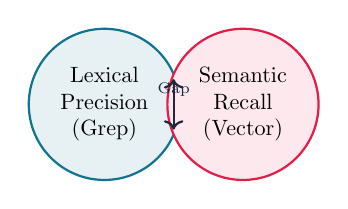
\begin{tikzpicture}[scale=0.8, every node/.style={transform shape}]
                \draw[thick, draw=secondary, fill=secondary!10] (0,0) circle (1.2cm) node[align=center] {Lexical\\Precision\\(Grep)};
                \draw[thick, draw=accent, fill=accent!10] (2.2,0) circle (1.2cm) node[align=center] {Semantic\\Recall\\(Vector)};
                \draw[<->, thick, primary] (1.1, 0.4) -- node[above, font=\scriptsize] {Gap} (1.1, -0.4);
            \end{tikzpicture}
        \end{column}
    \end{columns}
\end{frame}

% Slide 4: Why We Propose LQE
\begin{frame}{Why We Propose LQE (Lexical Query Expansion)}
    \begin{itemize}
        \item \textbf{Semantic Recall + Lexical Precision}: A lightweight LLM middleware step inside the harness expands semantic concepts into regex alternation groups (e.g., \texttt{vehicle} $\to$ \texttt{(sedan|coupe|suv|...)}).
        \item \textbf{Semantic Entity Locking}: Regex acts as a strict lexical filter, blocking vector search distractors (like apparel buying actions) by matching only specified category members.
        \item \textbf{Cognitive Offloading}: Offloads query planning from the main agent to the harness middleware, avoiding agent collapse on smaller backbones.
        \item \textbf{Zero-Index Infrastructure}: Reaps the benefits of semantic search directly on raw text files with zero embedding or vector database overhead.
    \end{itemize}
\end{frame}

% Slide 5: Proposed Solution
\begin{frame}[fragile]{Proposed Solution: Lexical Query Expansion (LQE)}
    \begin{center}
        \textbf{Harness-Level Regex Query Synthesis Loop}
        \vskip 1.5em
        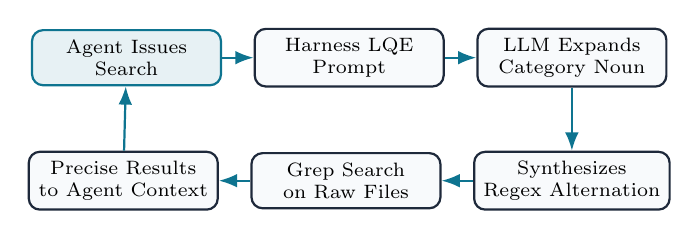
\begin{tikzpicture}[
            node distance=0.8cm and 0.4cm,
            stepnode/.style={draw=primary, thick, rounded corners, fill=background, align=center, font=\scriptsize, minimum height=0.7cm, minimum width=2.4cm},
            arrow/.style={-Latex, thick, secondary}
        ]
            \node[stepnode, fill=secondary!10, draw=secondary] (agent) {Agent Issues\\Search};
            \node[stepnode, right=of agent] (harness) {Harness LQE\\Prompt};
            \node[stepnode, right=of harness] (llm) {LLM Expands\\Category Noun};
            \node[stepnode, below=of llm] (regex) {Synthesizes\\Regex Alternation};
            \node[stepnode, left=of regex] (grep) {Grep Search\\on Raw Files};
            \node[stepnode, left=of grep] (results) {Precise Results\\to Agent Context};
            
            \draw [arrow] (agent) -- (harness);
            \draw [arrow] (harness) -- (llm);
            \draw [arrow] (llm) -- (regex);
            \draw [arrow] (regex) -- (grep);
            \draw [arrow] (grep) -- (results);
            \draw [arrow] (results) -- (agent);
        \end{tikzpicture}
    \end{center}
    \vskip 0.5em
    \begin{lstlisting}[caption=LQE Abstract Middleware Pipeline]
Agent issues Search -> [Harness LQE Prompt] -> LLM Synthesizes regex -> Grep search on raw files
    \end{lstlisting}
\end{frame}

% Slide 6: How the Benchmark Dataset is Created
\begin{frame}{How the Benchmark Dataset is Created}
    \textbf{Programmatic Dialogue Generation (Burying a Needle in a Haystack)}
    \vskip 1em
    \begin{enumerate}
        \item \textbf{Define Categories \& Templates}:
              \begin{itemize}
                  \item \textit{Category}: \texttt{vehicle} (Target item: \texttt{sedan})
                  \item \textit{Oracle Template}: \texttt{"The user purchased a \{color\} \{item\} yesterday."}
                  \item \textit{Synonym Query}: \texttt{"What color vehicle did the user buy?"} (forces vocabulary mismatch)
              \end{itemize}
        \item \textbf{Generate the Oracle (``The Needle''}):
              \begin{itemize}
                  \item Pick random attributes: \textit{emerald} and \textit{sedan}.
                  \item \textit{Oracle Turn}: \texttt{"[User]: The user purchased a emerald sedan yesterday."}
              \end{itemize}
        \item \textbf{Mix in Distractors (``The Haystack''}):
              \begin{itemize}
                  \item \textit{General}: \texttt{"The weather was quite nice today, perfect for walking."}
                  \item \textit{Same-Category}: \texttt{"The user was looking at a blue motorcycle online."}
                  \item \textit{Action-Overlap}: \texttt{"The user bought a matching white trenchcoat for the party."}
              \end{itemize}
        \item \textbf{Shuffle, Format, \& Noise Sweeps}: Distribute turns and scale noise levels (10, 20, 35).
    \end{enumerate}
\end{frame}

% Slide 7: Pilot Results
\begin{frame}{Pilot Results: LQE-Grep vs. Vector vs. Grep}
    \begin{columns}[T]
        \begin{column}{0.48\textwidth}
            \textbf{Accuracy \& Context Footprint (Qwen2.5-1.5B)}
            \vskip 0.8em
            \centering
            \small
            \begin{tabular}{llrr}
                \toprule
                \textbf{Noise} & \textbf{Method} & \textbf{Accuracy} & \textbf{Tokens} \\
                \midrule
                10 Dist. & Vanilla Grep & 0.0\% & 5.7 \\
                        & Vector Search & 33.3\% & 42.5 \\
                        & \textbf{LQE-Grep} & \textbf{83.3\%} & \textbf{45.7} \\
                \midrule
                20 Dist. & Vanilla Grep & 0.0\% & 8.5 \\
                        & Vector Search & 0.0\% & 42.5 \\
                        & \textbf{LQE-Grep} & \textbf{83.3\%} & \textbf{62.0} \\
                \midrule
                35 Dist. & Vanilla Grep & 0.0\% & 8.0 \\
                        & Vector Search & 0.0\% & 42.2 \\
                        & \textbf{LQE-Grep} & \textbf{100.0\%} & \textbf{63.7} \\
                \bottomrule
            \end{tabular}
        \end{column}
        \begin{column}{0.5\textwidth}
            \centering
            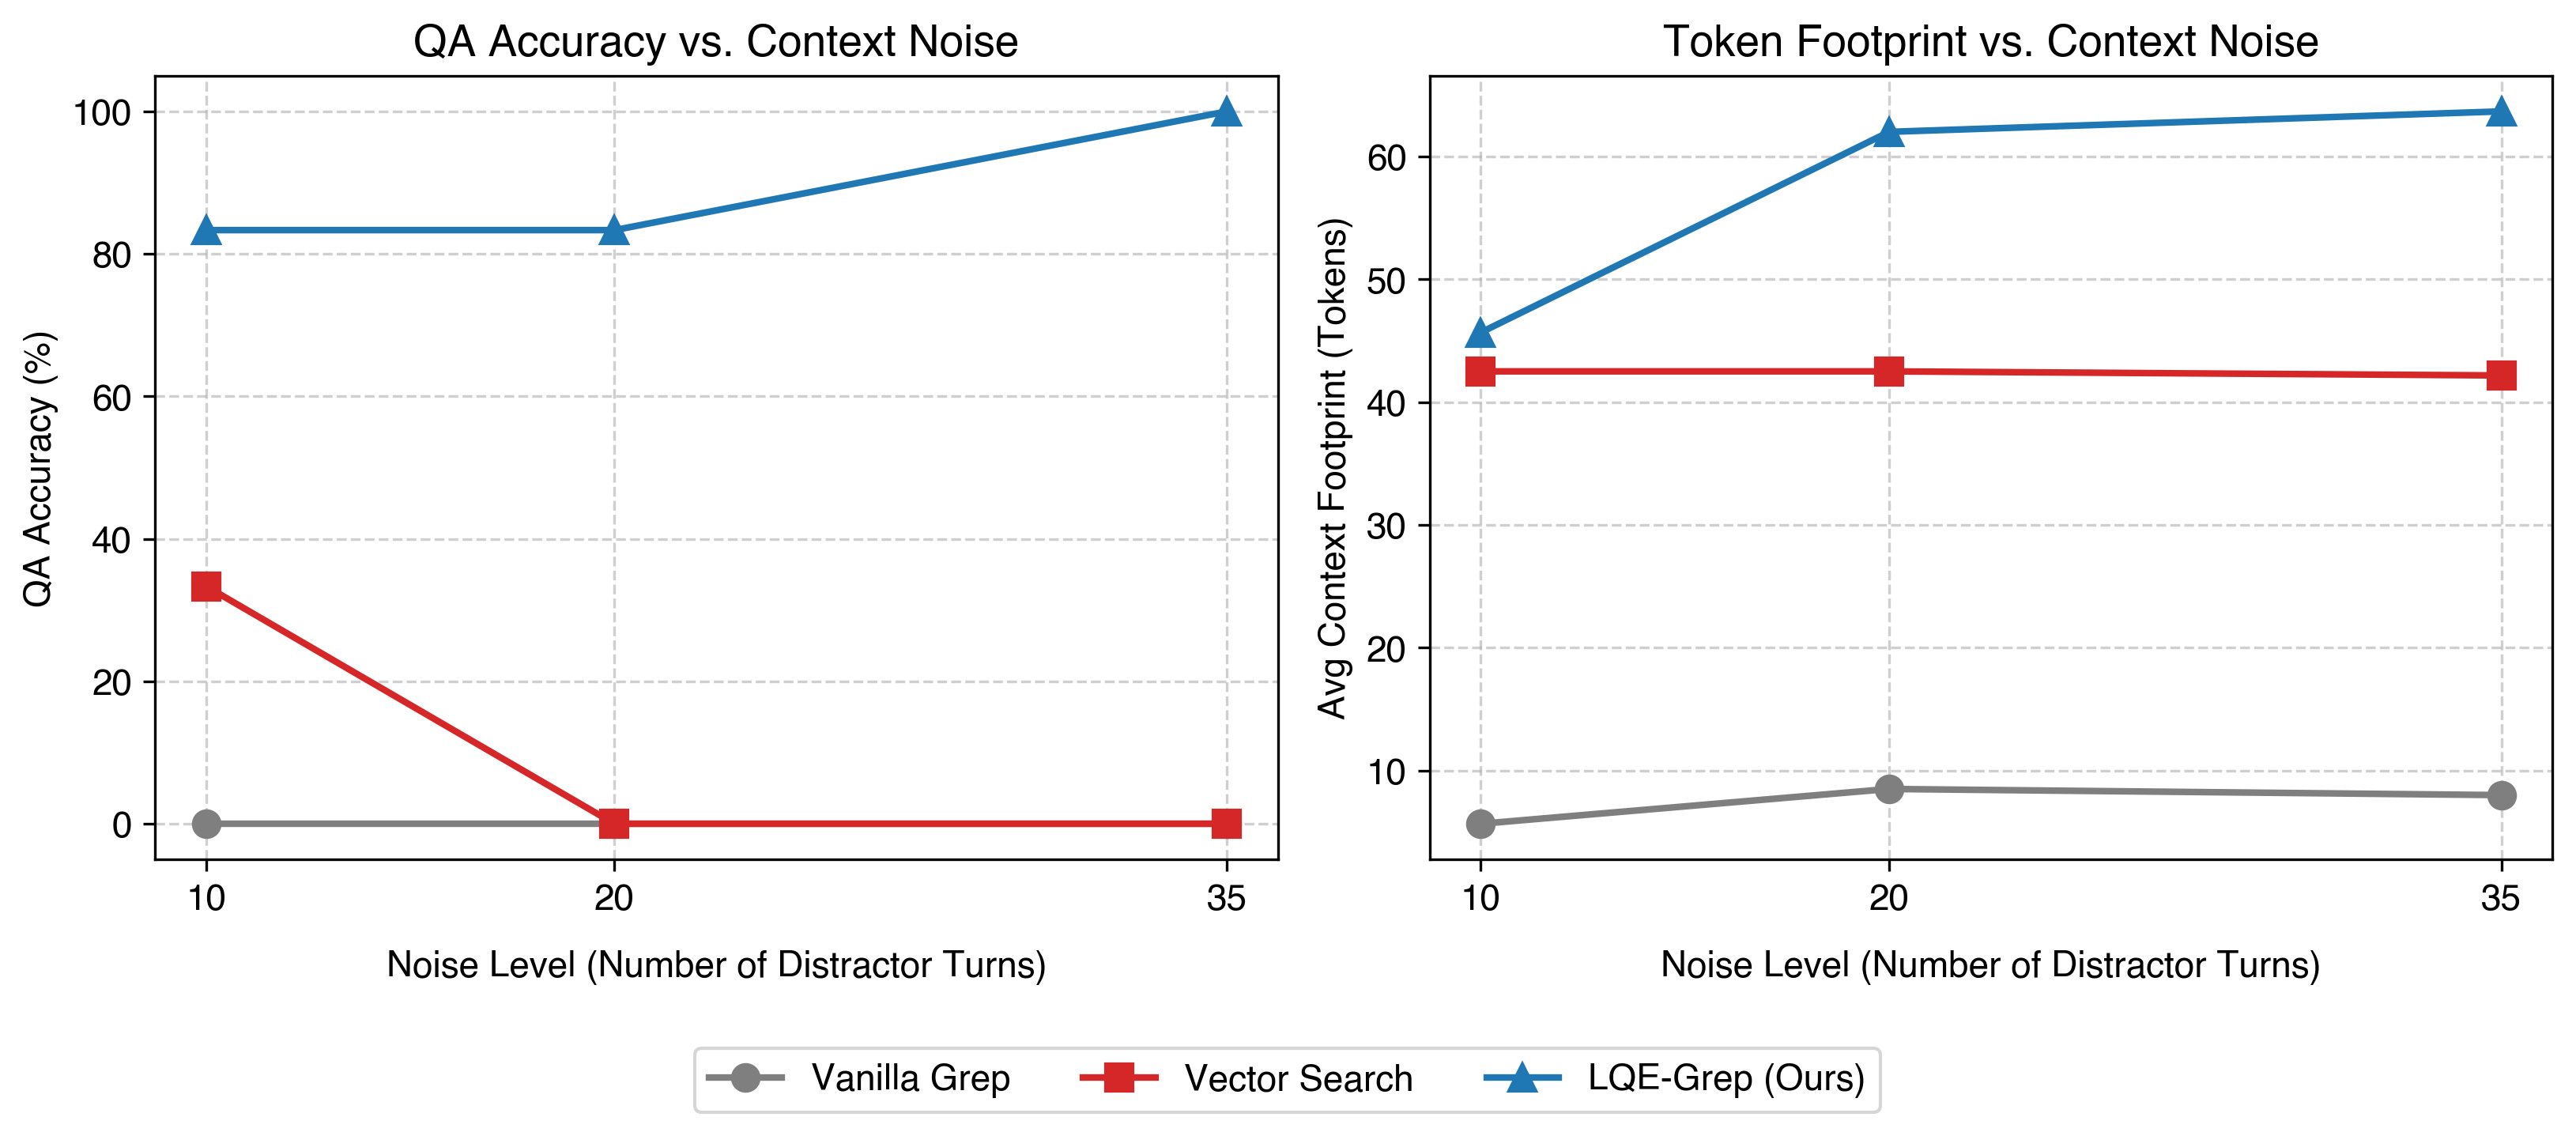
\includegraphics[width=\textwidth]{../evaluation_results.png}
        \end{column}
    \end{columns}
\end{frame}

% Slide 8: Real-World Benchmark: LongMemEval Evaluation
\begin{frame}{Real-World Benchmark: LongMemEval Evaluation}
    \begin{columns}[T]
        \begin{column}{0.5\textwidth}
            \textbf{Results on Real User-Assistant Conversations (~100k tokens)}
            \vskip 0.5em
            \centering
            \small
            \begin{tabular}{lrr}
                \toprule
                \textbf{Method} & \textbf{Accuracy} & \textbf{Avg. Tokens} \\
                \midrule
                Vanilla Grep & 55.7\% & 1,467.4 \\
                LQE-Grep (v1) & \textbf{65.7\%} & 4,697.3 \\
                LQE-Grep v2 (Ours) & 64.3\% & \textbf{4,191.0} \\
                Vector Search & 0.0\% & \textbf{64.4} \\
                \bottomrule
            \end{tabular}
            \vskip 0.8em
            \small
            * Evaluated on all 70 \texttt{single-session-user} queries from \texttt{longmemeval\_s\_cleaned.json}.
        \end{column}
        \begin{column}{0.48\textwidth}
            \begin{block}{The Truncation Bottleneck}
                \small
                \begin{itemize}
                    \item \textbf{Vector Search Fail}: Embedding 500+ turns was too slow, forcing truncation to the first 150 turns. The answer (in session 51) was missed entirely.
                    \item \textbf{Lexical Success}: Grep and LQE scanned all 500+ turns in milliseconds, capturing the needle.
                    \item \textbf{LQE v2 Optimization}: Filters local conversational noise (e.g. \textit{``name''}, \textit{``shop''}) using turn frequency filtering, saving 10.8\% tokens.
                \end{itemize}
            \end{block}
        \end{column}
    \end{columns}
\end{frame}

% Slide 9: Real-World Medical Benchmark: BEIR NFCorpus Evaluation
\begin{frame}{Real-World Medical Benchmark: BEIR NFCorpus Evaluation}
    \begin{columns}[T]
        \begin{column}{0.5\textwidth}
            \textbf{Zero-Shot Document Retrieval (Success@3) on Haystack of 50}
            \vskip 0.5em
            \centering
            \small
            \begin{tabular}{lrr}
                \toprule
                \textbf{Method} & \textbf{Success@3} & \textbf{Avg. Tokens} \\
                \midrule
                Vanilla Grep & 50.42\% & 1,949.6 \\
                LQE-Grep (v1) & 56.30\% & 5,689.8 \\
                LQE-Grep v2 (Ours) & \textbf{57.98\%} & \textbf{3,182.3} \\
                Vector Search & 15.13\% & N/A \\
                \bottomrule
            \end{tabular}
            \vskip 0.8em
            \small
            * Evaluated on all 323 test queries comparing patient-written terms to medical documents.
        \end{column}
        \begin{column}{0.48\textwidth}
            \begin{block}{The Precision Gap}
                \small
                \begin{itemize}
                    \item \textbf{Vector Search Fail}: Only 15.13\% Success@3 because embeddings blur the lines between related concepts (e.g. retrieving leukemia papers for *"Dragon's Blood"*).
                    \item \textbf{Lexical Precision}: Grep and LQE restrict matching to actual entity classes. LQE v2 global Document Frequency (DF) filtering cuts token inflation by 44.1\%.
                \end{itemize}
            \end{block}
        \end{column}
    \end{columns}
\end{frame}

% Slide 10: Insights
\begin{frame}{Insights: Semantic Entity Locking}
    \begin{columns}[T]
        \begin{column}{0.48\textwidth}
            \begin{block}{Why Vector Search Failed}
                \small
                Vector search is confused by \textbf{action template overlap}. When the query is \textit{``What color vehicle did the user buy?''}, it retrieves:
                \vskip 0.5em
                \texttt{[User]: The user bought a matching white trenchcoat for the party.}
                \vskip 0.5em
                Because \textit{``bought''} shares semantic overlaps with buying actions, vector search prioritizes sentence structure over the target entity category.
            \end{block}
        \end{column}
        \begin{column}{0.48\textwidth}
            \begin{block}{Why LQE-Grep Succeeded}
                \small
                The LLM expands \textit{``vehicle''} to a regex alternation like \texttt{(sedan|coupe|motorcycle|suv|truck|...)}.
                \vskip 0.5em
                The regex acts as an absolute \textbf{lexical filter}, forcing the tool to match only literal matching entity classes and completely ignoring action overlap.
            \end{block}
        \end{column}
    \end{columns}
\end{frame}

% Slide 10b: LongMemEval Case Study
\begin{frame}{Case Study: LongMemEval Retrieval}
    \begin{block}{Vocabulary Match vs. Context Truncation}
        \small
        \textbf{Query}: \textit{``How many shirts did I pack for my 5-day trip to Costa Rica?''} \hfill \textbf{Ground Truth}: 7
        \vskip 0.5em
        \textbf{Target Dialogue Turn}: 
        \texttt{[User]: ...on my last trip to Costa Rica, I brought 7 shirts and 5 pairs of shorts...}
    \end{block}
    \vskip 0.5em
    \begin{columns}[T]
        \begin{column}{0.48\textwidth}
            \begin{block}{LQE v2 Expansion \& Matching}
                \small
                \begin{itemize}
                    \item \textbf{LQE v2 Regex}: \\
                    \texttt{(costa|rica|trip|shirts|pack|travel|clothing|apparel|vacation)}
                    \item Matches target synonyms at native search speeds.
                    \item Filters local turn-frequency noise, saving 10.8\% context.
                \end{itemize}
            \end{block}
        \end{column}
        \begin{column}{0.48\textwidth}
            \begin{block}{Grep and Vector Behaviors}
                \small
                \begin{itemize}
                    \item \textbf{Vanilla Grep}: Strict match fails if query keywords (e.g. \textit{``pack''}, \textit{``shirts''}) are rephrased as \textit{``luggage''} or \textit{``tops''}.
                    \item \textbf{Vector Search}: Fails (0\% accuracy) because embedding 500+ turns exceeds context lengths, forcing aggressive truncation that drops the target session.
                \end{itemize}
            \end{block}
        \end{column}
    \end{columns}
\end{frame}

% Slide 10c: BEIR NFCorpus Case Study
\begin{frame}{Case Study: BEIR NFCorpus Medical Search}
    \begin{block}{Resolving Technical Synonyms \& Term Pruning}
        \small
        \textbf{Query}: \textit{``Phytates for the Treatment of Cancer''} \hfill \textbf{Target Doc (MED-2568)}
        \vskip 0.5em
        \textbf{Abstract Title}: \textit{IP6: a novel anti-cancer agent.} \\
        \textbf{Abstract Text}: \textit{Inositol hexaphosphate (InsP6 or IP6) is ubiquitous... A striking anti-cancer action of IP6 has been demonstrated both in vivo and in vitro...}
    \end{block}
    \vskip 0.5em
    \begin{columns}[T]
        \begin{column}{0.48\textwidth}
            \begin{block}{LQE v2 vs. LQE v1 Regex}
                \small
                \begin{itemize}
                    \item \textbf{LQE v1}: \texttt{(phytates|phyticacid|...|health|wellness)} (pulls in massive distractor documents containing the generic term \textit{``health''}).
                    \item \textbf{LQE v2 (DF-Pruned)}: \\
                    \texttt{(phytates|phyticacid|phytochemicals|antioxidants|anti-cancer|wellness)}
                    \item Pruning \textit{``health''} saves 44.1\% tokens.
                \end{itemize}
            \end{block}
        \end{column}
        \begin{column}{0.48\textwidth}
            \begin{block}{Grep and Vector Behaviors}
                \small
                \begin{itemize}
                    \item \textbf{Vanilla Grep}: Fails because \textit{``phytates''} is not explicitly present in the abstract (only its chemical synonym \textit{``Inositol hexaphosphate''}).
                    \item \textbf{Vector Search}: Fails (15.13\% success) due to semantic blurring, retrieving generic cancer papers instead of IP6.
                \end{itemize}
            \end{block}
        \end{column}
    \end{columns}
\end{frame}

% Slide 11: Critical Optimization: Word Boundaries
\begin{frame}{Critical Optimization: Word Boundaries}
    \begin{columns}[T]
        \begin{column}{0.5\textwidth}
            \textbf{The Substring Collision Bug}
            \vskip 0.5em
            \begin{itemize}
                \item Early query expansion for \textit{vehicle} included \textbf{``car''}.
                \item Matched distractor substrings: \textbf{\color{accent}car}diologist, \textbf{\color{accent}car}digan.
                \item Context flooded with false positives $\to$ accuracy dropped to \textbf{16.67\%}.
            \end{itemize}
            \vskip 0.8em
            \textbf{The Word Boundary Fix}
            \begin{itemize}
                \item Wrap all LQE regex strings in boundaries (\texttt{\textbackslash b}):
                      \texttt{\textbackslash b(sedan|coupe|...|car)\textbackslash b}
                \item Restores accuracy instantly to \textbf{100.0\%}.
            \end{itemize}
        \end{column}
        \begin{column}{0.45\textwidth}
            \begin{block}{Visual Representation}
                \vskip 0.5em
                \centering
                \small
                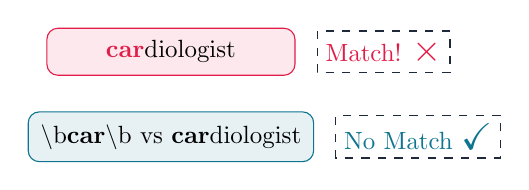
\begin{tikzpicture}[scale=0.9, every node/.style={transform shape}]
                    % Word: Cardiologist
                    \node[draw=accent, fill=accent!10, rounded corners, inner sep=5pt, minimum width=3.5cm] (w1) at (0, 1.2) {\textbf{\color{accent}car}diologist};
                    \node[draw=primary, dashed, right=0.3cm of w1, text=accent] {Match! \hfill \scalebox{1.5}{$\mathbf{\times}$}};
                    
                    % Fixed Word: \b car \b vs cardiologist
                    \node[draw=secondary, fill=secondary!10, rounded corners, inner sep=5pt, minimum width=3.5cm] (w2) at (0, 0) {\textbackslash b\textbf{car}\textbackslash b vs \textbf{car}diologist};
                    \node[draw=primary, dashed, right=0.3cm of w2, text=secondary] {No Match \hfill \scalebox{1.5}{$\mathbf{\checkmark}$}};
                \end{tikzpicture}
            \end{block}
        \end{column}
    \end{columns}
\end{frame}

% Slide 12: Scaled Plan & Next Steps
\begin{frame}{Scaled Plan \& Next Steps}
    \begin{enumerate}
        \item \textbf{Stop-Word \& Common-Word Filtering}:
              \begin{itemize}
                  \item Optimize LQE query expansion to prune overly broad terms (like \textit{``name''} or \textit{``shop''}) that cause high token recall in large corpora.
              \end{itemize}
              \vskip 0.5em
        \item \textbf{Scale Real-World Evaluation}:
              \begin{itemize}
                  \item Evaluate on the full 500-question LongMemEval dataset and the complete 3,000+ document BEIR NFCorpus benchmark.
              \end{itemize}
              \vskip 0.5em
        \item \textbf{Draft Paper Layout}:
              \begin{itemize}
                  \item Present LQE-Grep as a compute-efficient, zero-index alternative to RAG for dynamic environments.
                  \item Detail how the compute complexity of embedding-based search forces truncation in long-context, failing where lexical search succeeds.
              \end{itemize}
    \end{enumerate}
\end{frame}

\end{document}
